\documentclass[aspectratio=169]{beamer}

% Theme Selection - Using Madrid (professional and clean)
\usetheme{Madrid}
\usecolortheme{default}

% AUEB Color Customization (uncomment and adjust if you have official colors)
% \definecolor{auebblue}{RGB}{0,51,102}  % Example AUEB blue - adjust as needed
% \setbeamercolor{structure}{fg=auebblue}
% \setbeamercolor{palette primary}{bg=auebblue,fg=white}
% \setbeamercolor{palette secondary}{bg=auebblue!80,fg=white}
% \setbeamercolor{palette tertiary}{bg=auebblue!60,fg=white}

\usepackage{graphicx}
\usepackage{booktabs}

% Title Page Information
\title{PISA 2018 Analysis}
\subtitle{Greece's Educational Performance in Global Context}
\author{Michael Theophanopoulos}
\institute{Athens University of Economics and Business (AUEB)}
\date{\today}

% Add AUEB logo (uncomment when you have the logo file)
% \titlegraphic{\includegraphics[width=3cm]{aueb_logo.png}}

\begin{document}

% Title Slide
\begin{frame}
\titlepage
\end{frame}

% Table of Contents
\begin{frame}{Outline}
\tableofcontents
\end{frame}

% Section 1: Global Position
\section{Greece's Global Position}

\begin{frame}{Greece in Global Context}
\begin{columns}
\column{0.5\textwidth}

\includegraphics[width=\textwidth]{plots/plot2.png}

\column{0.5\textwidth}
\begin{itemize}
\item Greece ranks \#46/80 globally with an overall score of 458, significantly below the global average
\item There is a massive 124-point gap between Greece and the top performer (B-S-J-Z China: 582)
\item The country is closer to the bottom 10 performers than to the top 10
\end{itemize}
\end{columns}
\end{frame}

\begin{frame}{Where Does Greece Stand Globally?}
\begin{columns}
\column{0.5\textwidth}
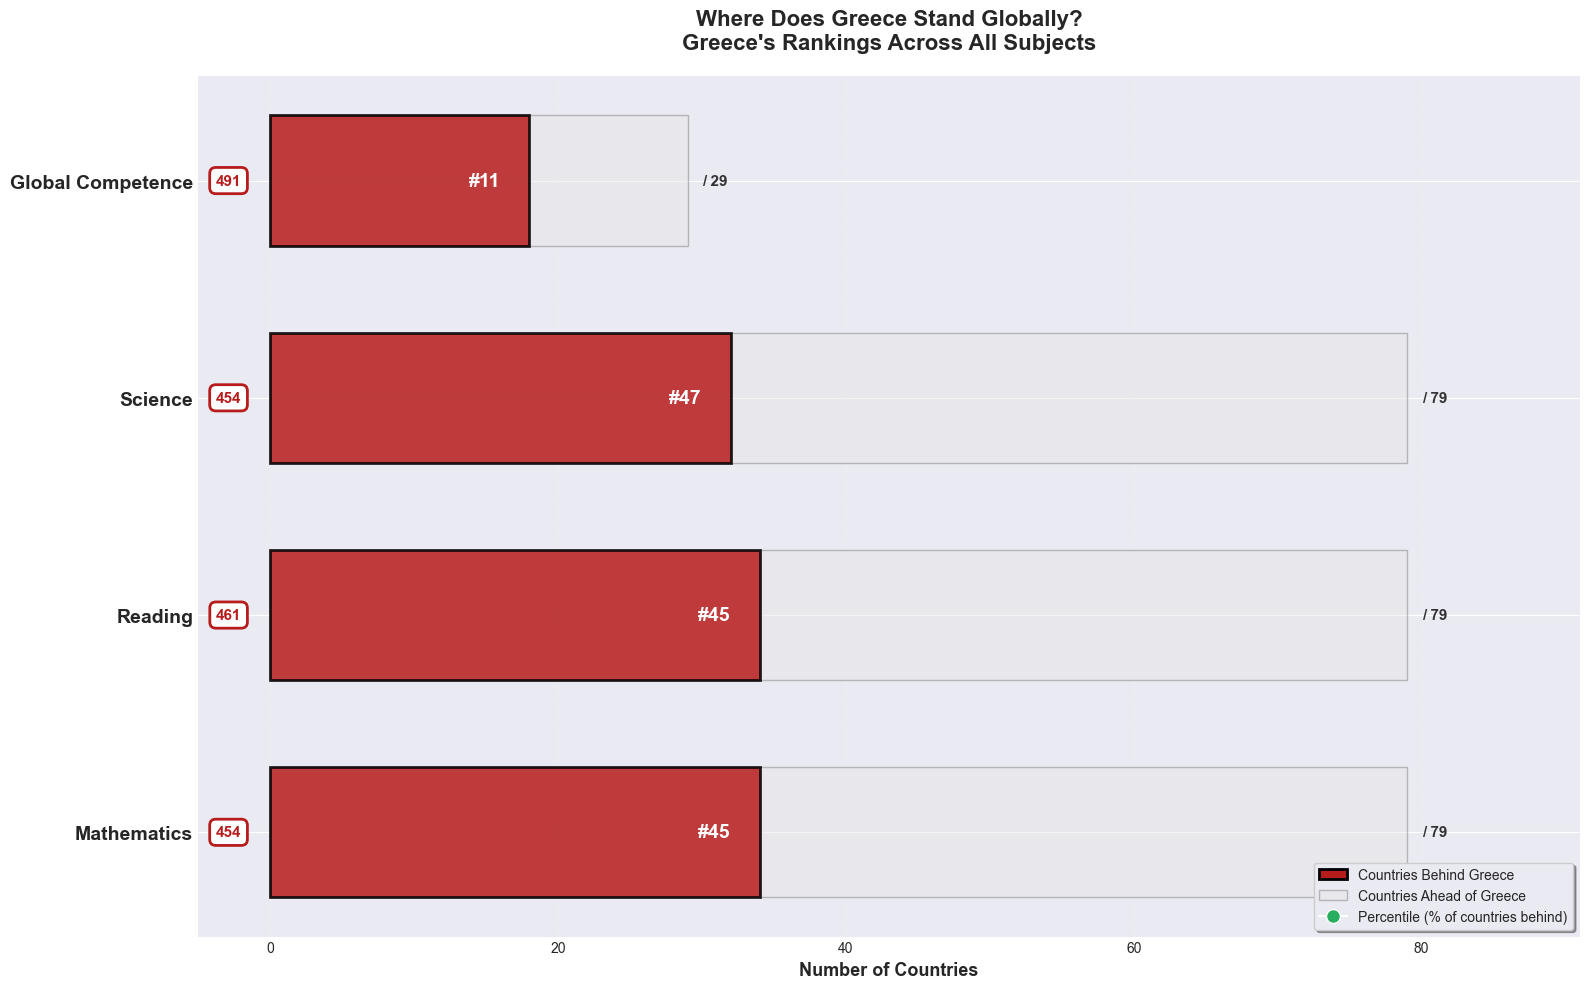
\includegraphics[width=\textwidth]{plots/plot10.png}

\column{0.5\textwidth}
\begin{itemize}
\item Greece's best performance is in Global Competence (\#11/29 countries, score 491)
\item In academic subjects the ranking is consistently low: \#45 in Mathematics and Reading, \#47 in Science
\item Clear dichotomy: exceptional global competence vs. weak academic performance
\end{itemize}
\end{columns}
\end{frame}

% Section 2: Regional Comparisons
\section{Regional \& Continental Comparisons}

\begin{frame}{Mediterranean \& Balkan Regional Comparison}
\begin{columns}
\column{0.5\textwidth}

\includegraphics[width=\textwidth]{plots/plot4.png}

\column{0.5\textwidth}
\begin{itemize}
\item Greece exceeds the regional average by $\sim$10 points in Global Competence (top regional performer)
\item In Mathematics it lags behind the regional average by $\sim$7 points
\item Large variation exists within the region (Spain at the top, Albania at the bottom)
\end{itemize}
\end{columns}
\end{frame}

\begin{frame}{Greece vs Continental Averages: Trend Analysis}
\begin{columns}
\column{0.5\textwidth}

\includegraphics[width=\textwidth]{plots/plot8.png}

\column{0.5\textwidth}
\begin{itemize}
\item Greece remains consistently below all continents except Africa across all subjects
\item The largest gap is with Oceania ($\sim$30-40 points) and Europe
\item Global Competence performance is the only highlight, approaching the Asian average
\end{itemize}
\end{columns}
\end{frame}

\begin{frame}{Greece vs Continental Averages: Detailed Breakdown}
\begin{columns}
\column{0.5\textwidth}

\includegraphics[width=\textwidth]{plots/plot7.png}

\column{0.5\textwidth}
\begin{itemize}
\item Detailed breakdown: Greece 454 (Math), 461 (Reading), 454 (Science), 491 (GLCM)
\item In all academic subjects Greece falls 20-30 points behind Europe
\item Greece's Global Competence score is between Asia and Europe, showing strong soft skills
\end{itemize}
\end{columns}
\end{frame}

% Section 3: Educational Inequality
\section{Educational Inequality \& Social Factors}

\begin{frame}{Educational Inequality Across Countries}
\begin{columns}
\column{0.5\textwidth}

\includegraphics[width=\textwidth]{plots/plot5.png}

\column{0.5\textwidth}
\begin{itemize}
\item Greece shows large internal inequality with a wide range between percentiles
\item Greece's median (458) is close to the global median but with greater dispersion
\item Mediterranean countries (Greece, Italy, Spain) exhibit similar inequality patterns
\end{itemize}
\end{columns}
\end{frame}

\begin{frame}{The Equality Test: Family Background Impact}
\begin{columns}
\column{0.5\textwidth}

\includegraphics[width=\textwidth]{plots/plot9.png}

\column{0.5\textwidth}
\begin{itemize}
\item Greece shows a 64-point difference between students with university-educated parents vs. less educated (ISCED 1)
\item It falls in the "inequality zone" below the equality line
\item Family background has a stronger impact in Greece than in countries like Estonia or Finland
\end{itemize}
\end{columns}
\end{frame}

\begin{frame}{The Parent Effect: Mother vs Father Education}
\begin{columns}
\column{0.5\textwidth}
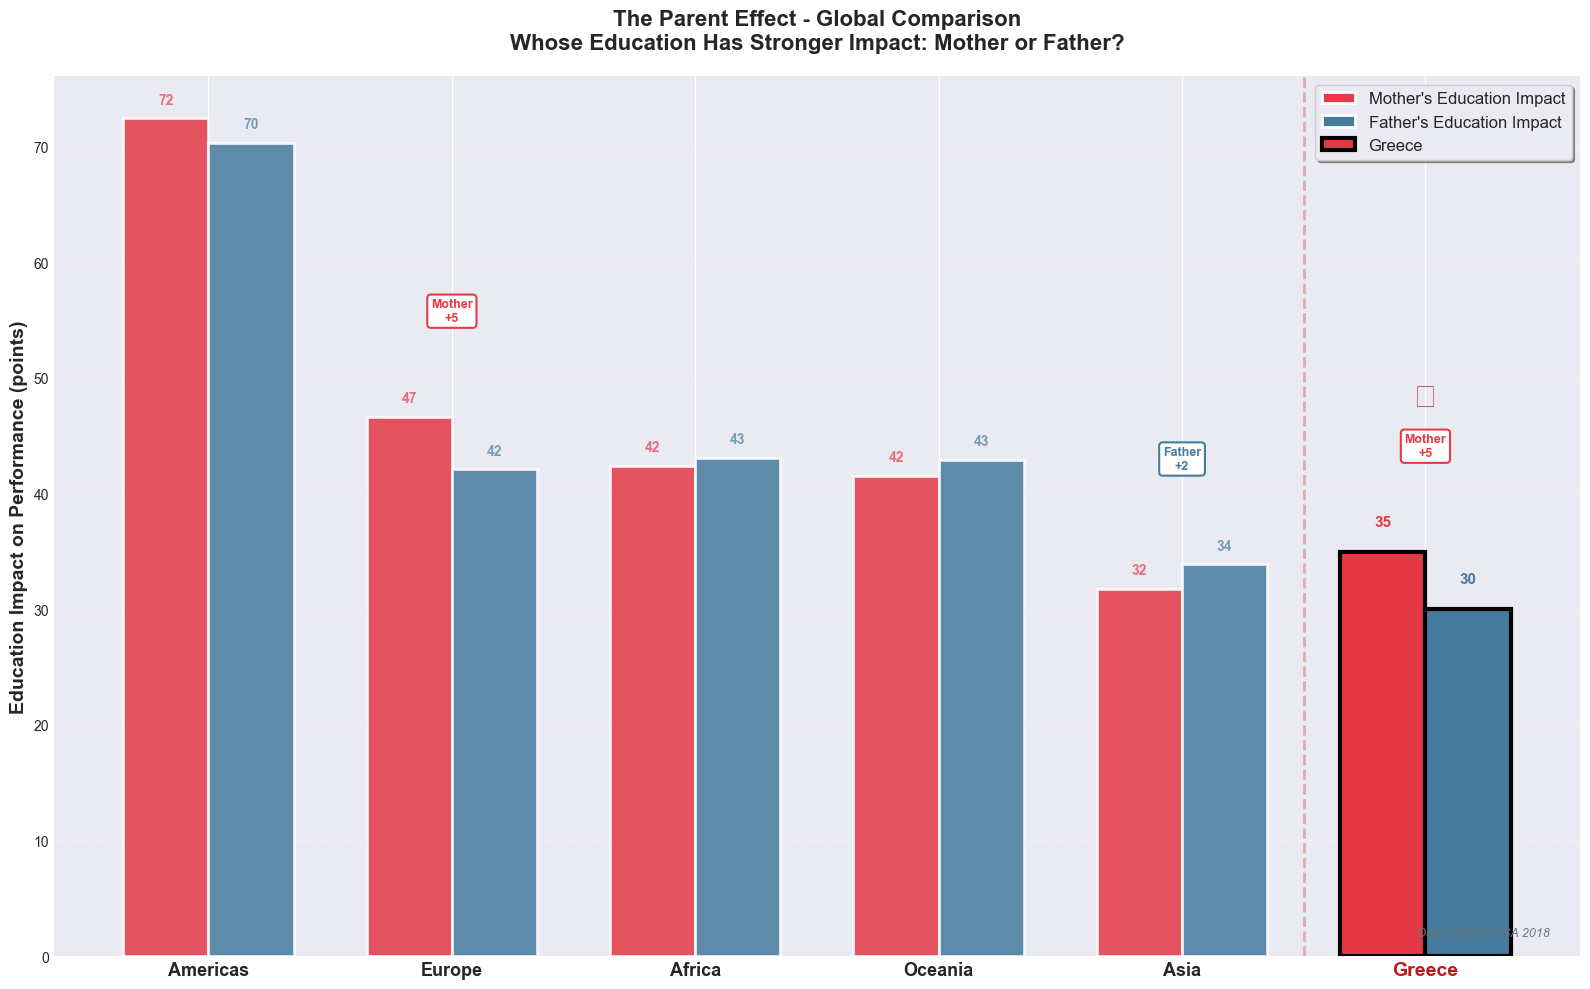
\includegraphics[width=\textwidth]{plots/plot11.png}

\column{0.5\textwidth}
\begin{itemize}
\item In Greece, mother's education has a stronger impact (+35 points) vs. father's (+30 points)
\item The +5 point difference favoring mothers is greater than the European trend
\item Both parental impacts are lower in Greece compared to other continents (Americas: 72-70)
\end{itemize}
\end{columns}
\end{frame}

% Section 4: Gender Analysis
\section{Gender Performance Analysis}

\begin{frame}{Gender Performance Gap in Mathematics}
\begin{columns}
\column{0.5\textwidth}

\includegraphics[width=\textwidth]{plots/plot1.png}

\column{0.5\textwidth}
\begin{itemize}
\item Greece is one of the few countries where girls outperform boys in mathematics (+1.5 points)
\item Contrasts with top performers (China, Singapore) where boys lead by 3-9 points
\item In bottom performers the gender gap favoring boys reaches 13 points (Saudi Arabia)
\end{itemize}
\end{columns}
\end{frame}

\begin{frame}{Gender Gap Distribution Patterns}
\begin{columns}
\column{0.5\textwidth}

\includegraphics[width=\textwidth]{plots/plot3.png}

\column{0.5\textwidth}
\begin{itemize}
\item In Greece, male-female distributions almost overlap, with a slight advantage for girls
\item Contrasts with bottom performers (Qatar, Saudi Arabia) where there's a massive -15 to -23 point gap
\item In top performers (China) boys have a +7.5 point advantage
\end{itemize}
\end{columns}
\end{frame}

\begin{frame}{Gender Performance Across Continents}
\begin{columns}
\column{0.5\textwidth}
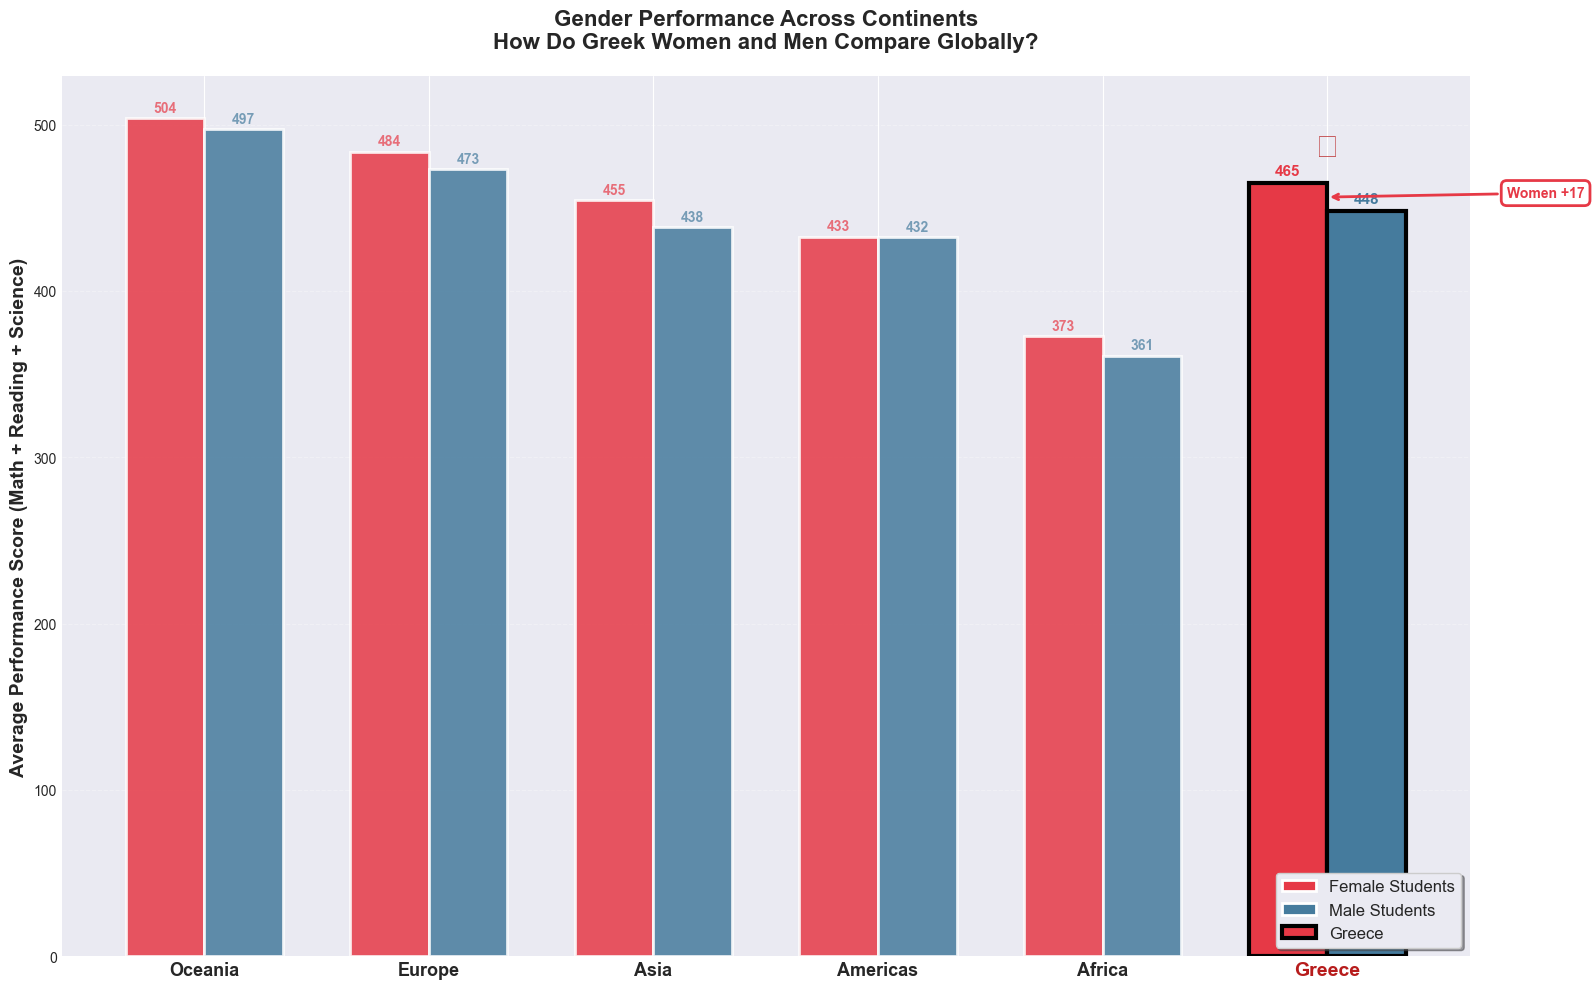
\includegraphics[width=\textwidth]{plots/plot12.png}

\column{0.5\textwidth}
\begin{itemize}
\item Greek female students (+17 points above males) exceed the global pattern
\item Girls lead in all continents, but Greece shows the largest gap
\item Overall performance (465 females, 448 males) remains below all continents except Africa
\end{itemize}
\end{columns}
\end{frame}

% Section 5: Academic vs Global Competence
\section{Academic vs Global Competence}

\begin{frame}{Academic vs Global Competence Landscape}
\begin{columns}
\column{0.5\textwidth}

\includegraphics[width=\textwidth]{plots/plot6.png}

\column{0.5\textwidth}
\begin{itemize}
\item Greece (rank \#46 academic, \#11 GLCM) is an outlier: low academic but exceptional global competence
\item Correlation 0.949 shows that typically academic and GLCM go together, but Greece breaks this pattern
\item Located in the "Low Academic, High GLCM - Hidden Strength" quadrant with only 2 other countries (6.9\%)
\end{itemize}
\end{columns}
\end{frame}

% Conclusion
\section{Conclusions}

\begin{frame}{Key Takeaways}
\begin{itemize}
\item \textbf{Global Position:} Greece ranks in the lower half globally (\#46/80), but excels in Global Competence (\#11/29)
\item \textbf{Regional Context:} Performance lags behind European averages by 20-30 points in academic subjects
\item \textbf{Educational Inequality:} Significant impact of family background (64-point gap), with mother's education showing stronger effect
\item \textbf{Gender Dynamics:} Greece shows a rare reversal with girls outperforming boys (+1.5 in Math, +17 overall)
\item \textbf{Hidden Strength:} Exceptional global competence despite weak academic scores suggests strong soft skills and cross-cultural awareness
\end{itemize}
\end{frame}

\begin{frame}[plain]
\centering
\Huge Thank You!\\[1em]
\large Questions?
\end{frame}

\end{document}
